% Book-only title page inspired by a hand-drawn engineering notebook.
\usepackage{tikz}
\usetikzlibrary{calc}

\definecolor{PolarisPaper}{HTML}{FFFFFF}
\definecolor{PolarisInk}{HTML}{332F2A}
\definecolor{PolarisGrid}{HTML}{EEEEEE}

\newfontfamily\PolarisTitleFont[
  Path=fonts/playfair-display/
]{PlayfairDisplay.ttf}

\makeatletter

\providecommand{\subtitle}[1]{}
\providecommand{\@subtitle}{}
\renewcommand{\subtitle}[1]{\gdef\@subtitle{#1}}

\newcommand{\PolarisDivider}{%
  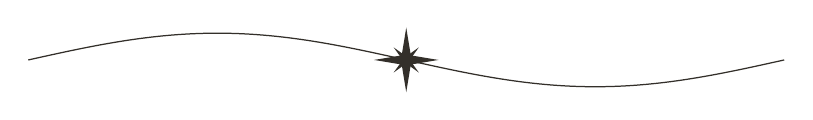
\begin{tikzpicture}[baseline=-0.55ex,x=1mm,y=1mm]
    \draw[
      draw=PolarisInk,
      line width=0.45pt,
      smooth,
      samples=121,
      domain=-48:48
    ] plot (\x,{-3.4*sin(180*\x/48)});

    \fill[PolarisInk]
      (0,4.1) -- (0.58,0.58) -- (4.1,0) -- (0.58,-0.58) --
      (0,-4.1) -- (-0.58,-0.58) -- (-4.1,0) -- (-0.58,0.58) -- cycle;
    \begin{scope}[rotate=45,scale=0.55]
      \fill[PolarisInk]
        (0,4.1) -- (0.58,0.58) -- (4.1,0) -- (0.58,-0.58) --
        (0,-4.1) -- (-0.58,-0.58) -- (-4.1,0) -- (-0.58,0.58) -- cycle;
    \end{scope}
  \end{tikzpicture}%
}

\newcommand{\PolarisCoverSketches}{%
  \begin{tikzpicture}[remember picture,overlay]
    \fill[PolarisPaper]
      (current page.south west) rectangle (current page.north east);

    \node[anchor=north west,inner sep=0]
      at ($(current page.north west)+(9mm,-9mm)$)
      {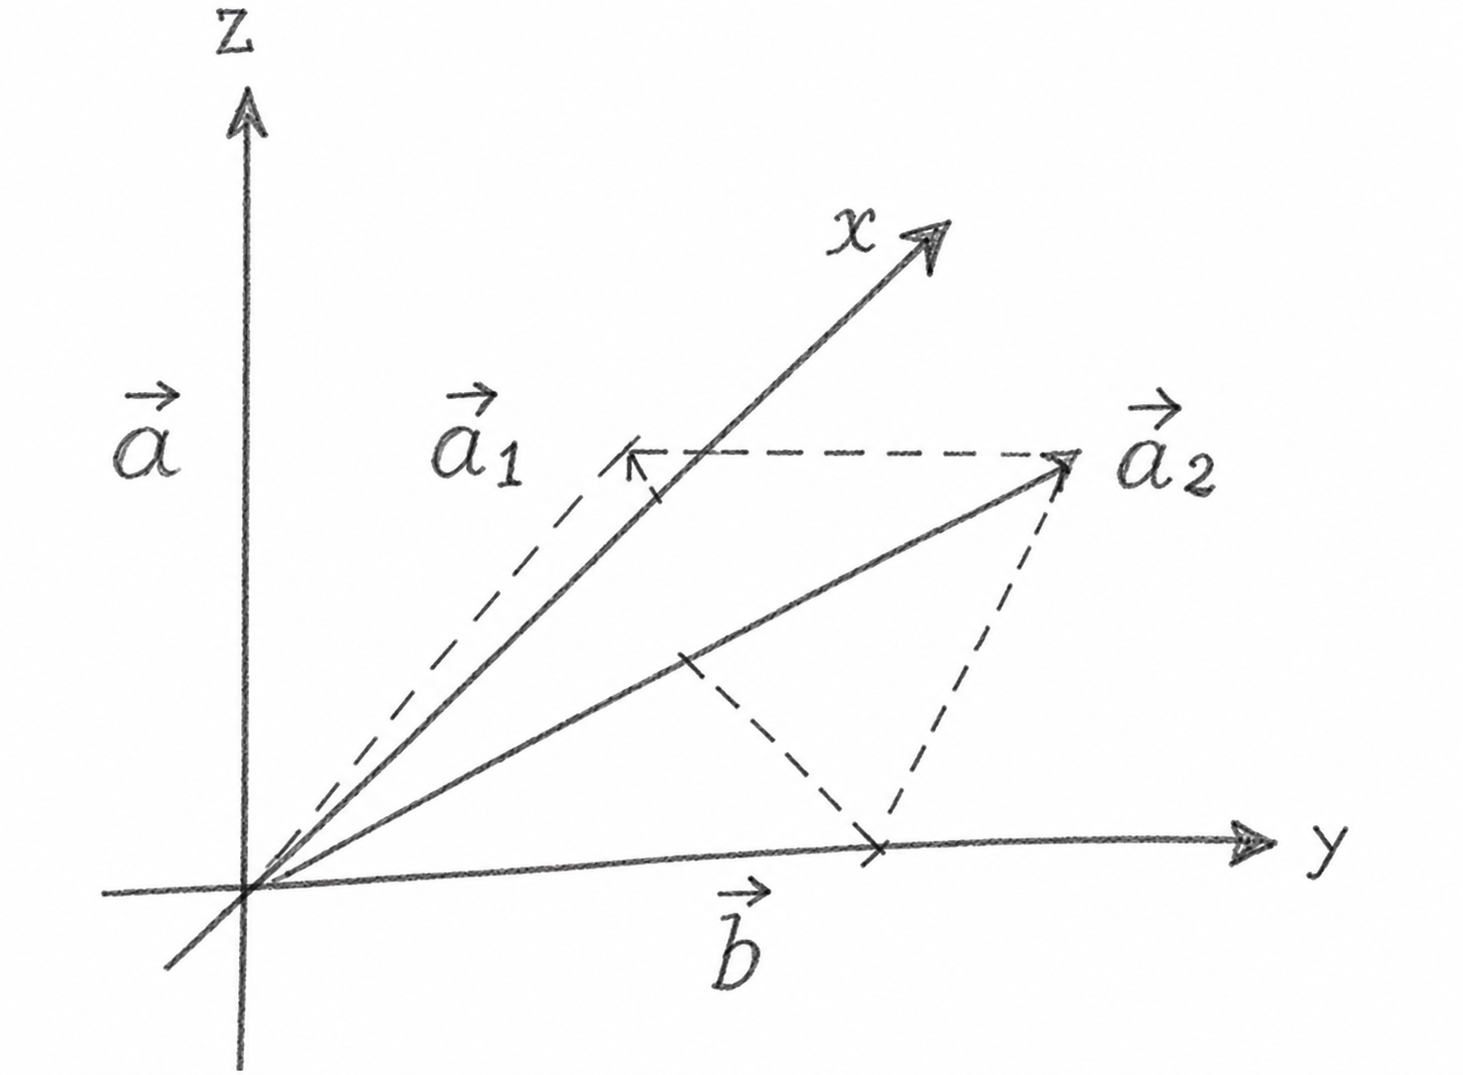
\includegraphics[width=0.39\paperwidth]{images/book-cover-top-left-white.png}};

    \node[anchor=north east,inner sep=0]
      at ($(current page.north east)+(-9mm,-9mm)$)
      {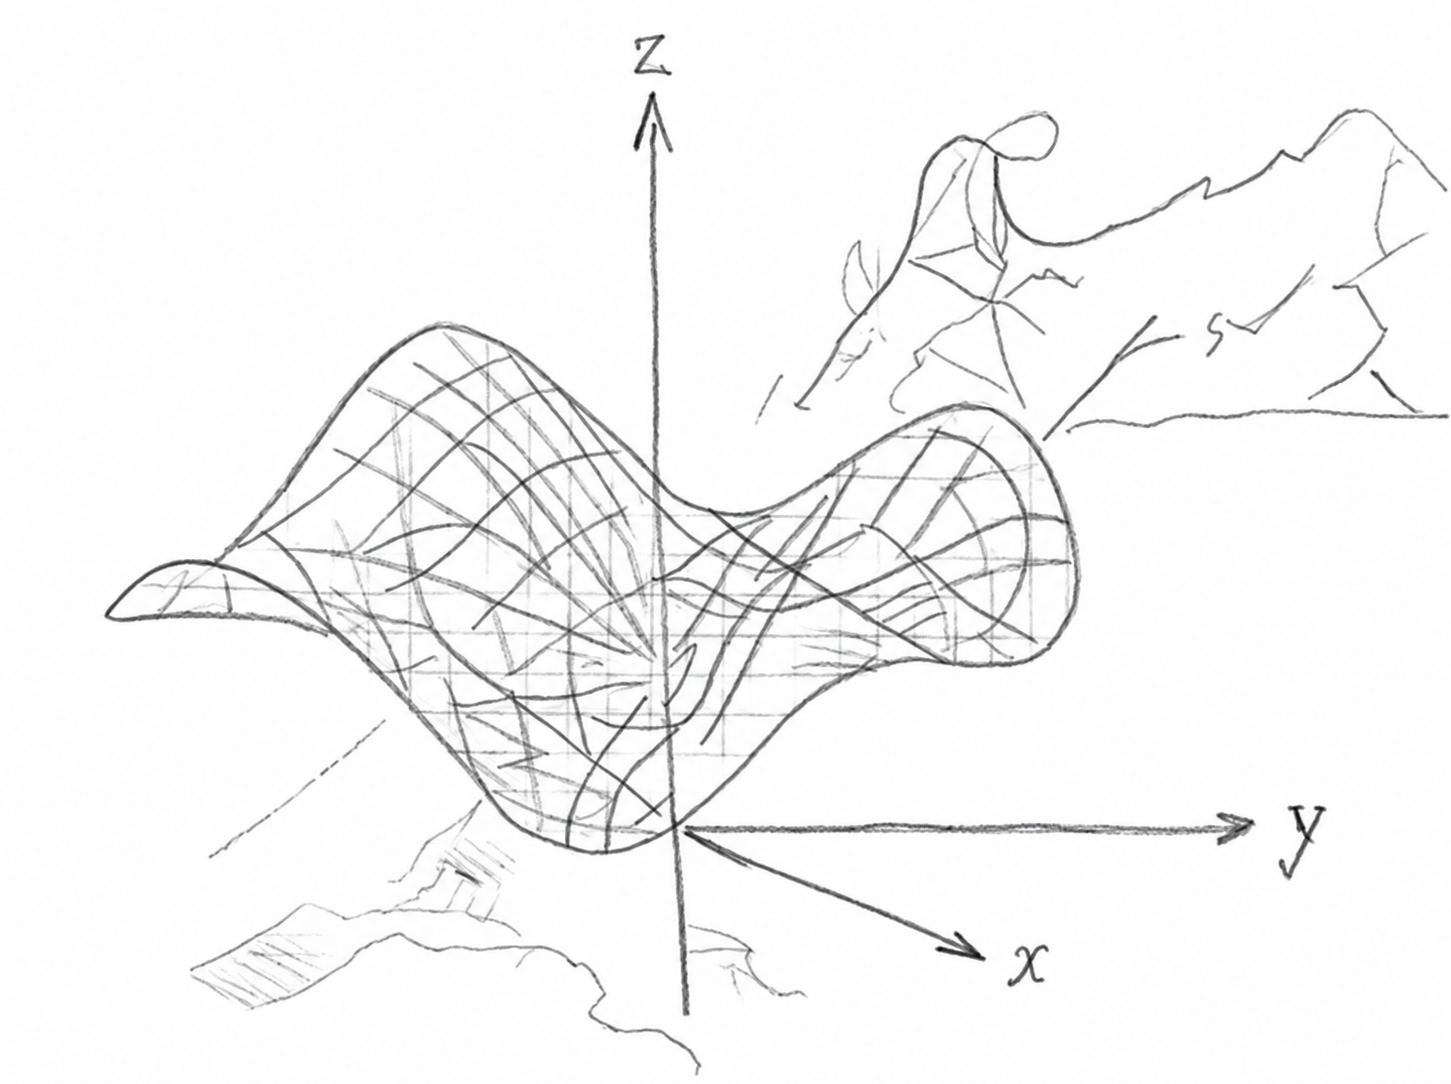
\includegraphics[width=0.39\paperwidth]{images/book-cover-top-right-white.png}};

    \node[anchor=south west,inner sep=0]
      at ($(current page.south west)+(9mm,9mm)$)
      {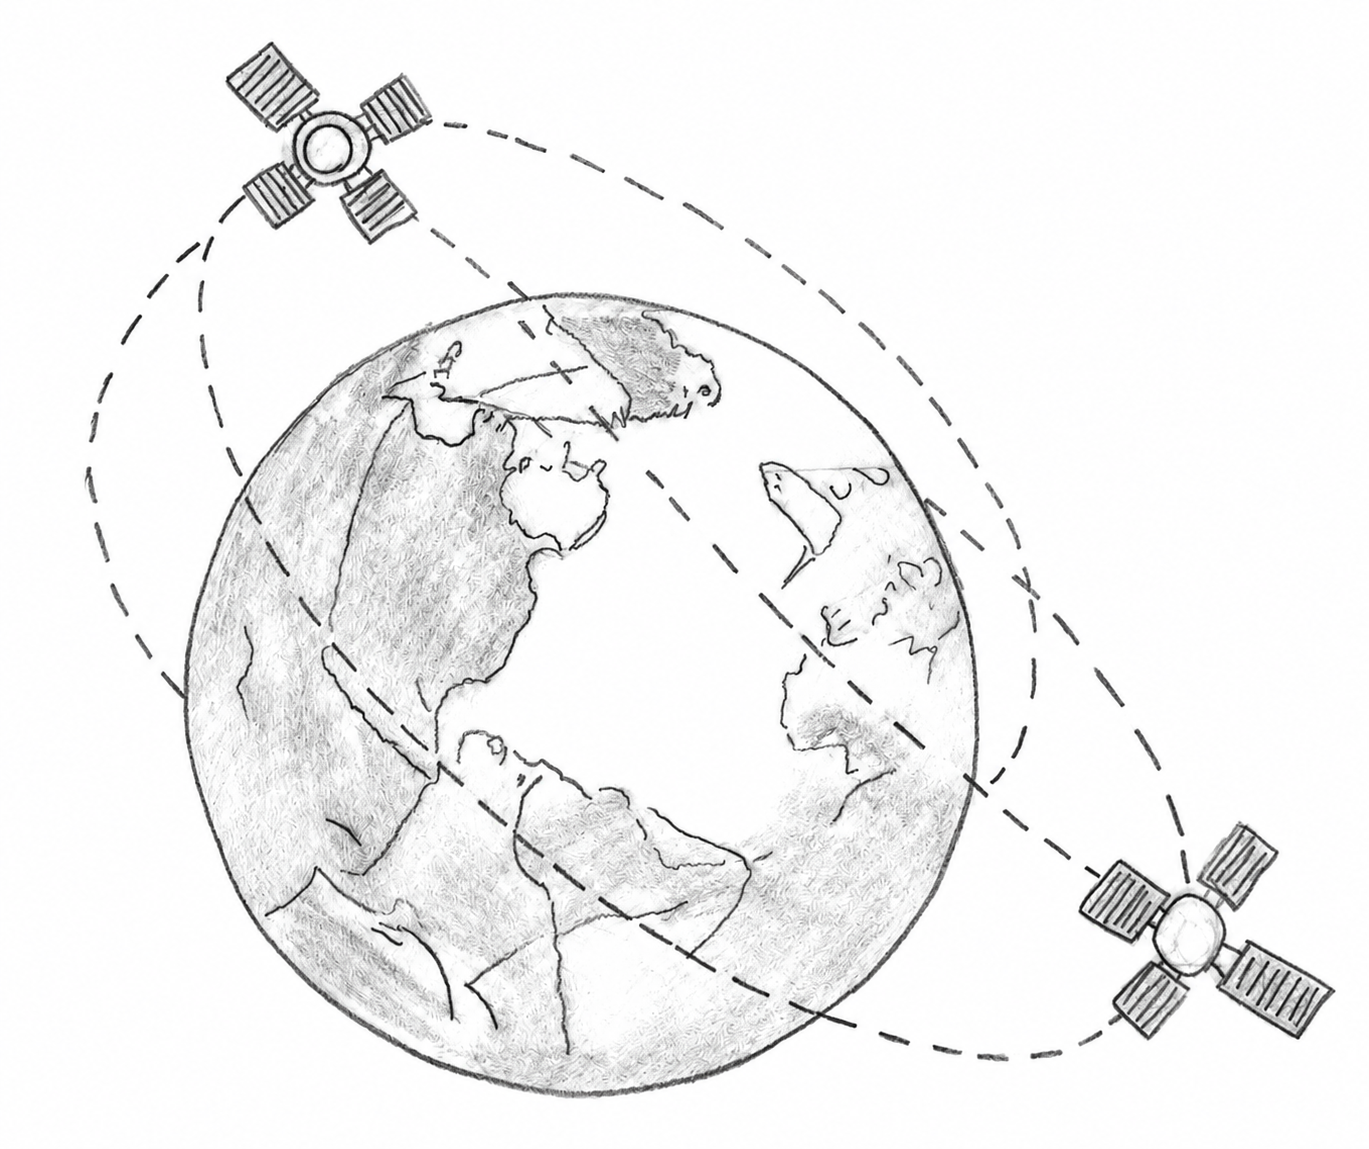
\includegraphics[width=0.39\paperwidth]{images/book-cover-bottom-left-title-white.png}};

    \node[anchor=south east,inner sep=0]
      at ($(current page.south east)+(-9mm,9mm)$)
      {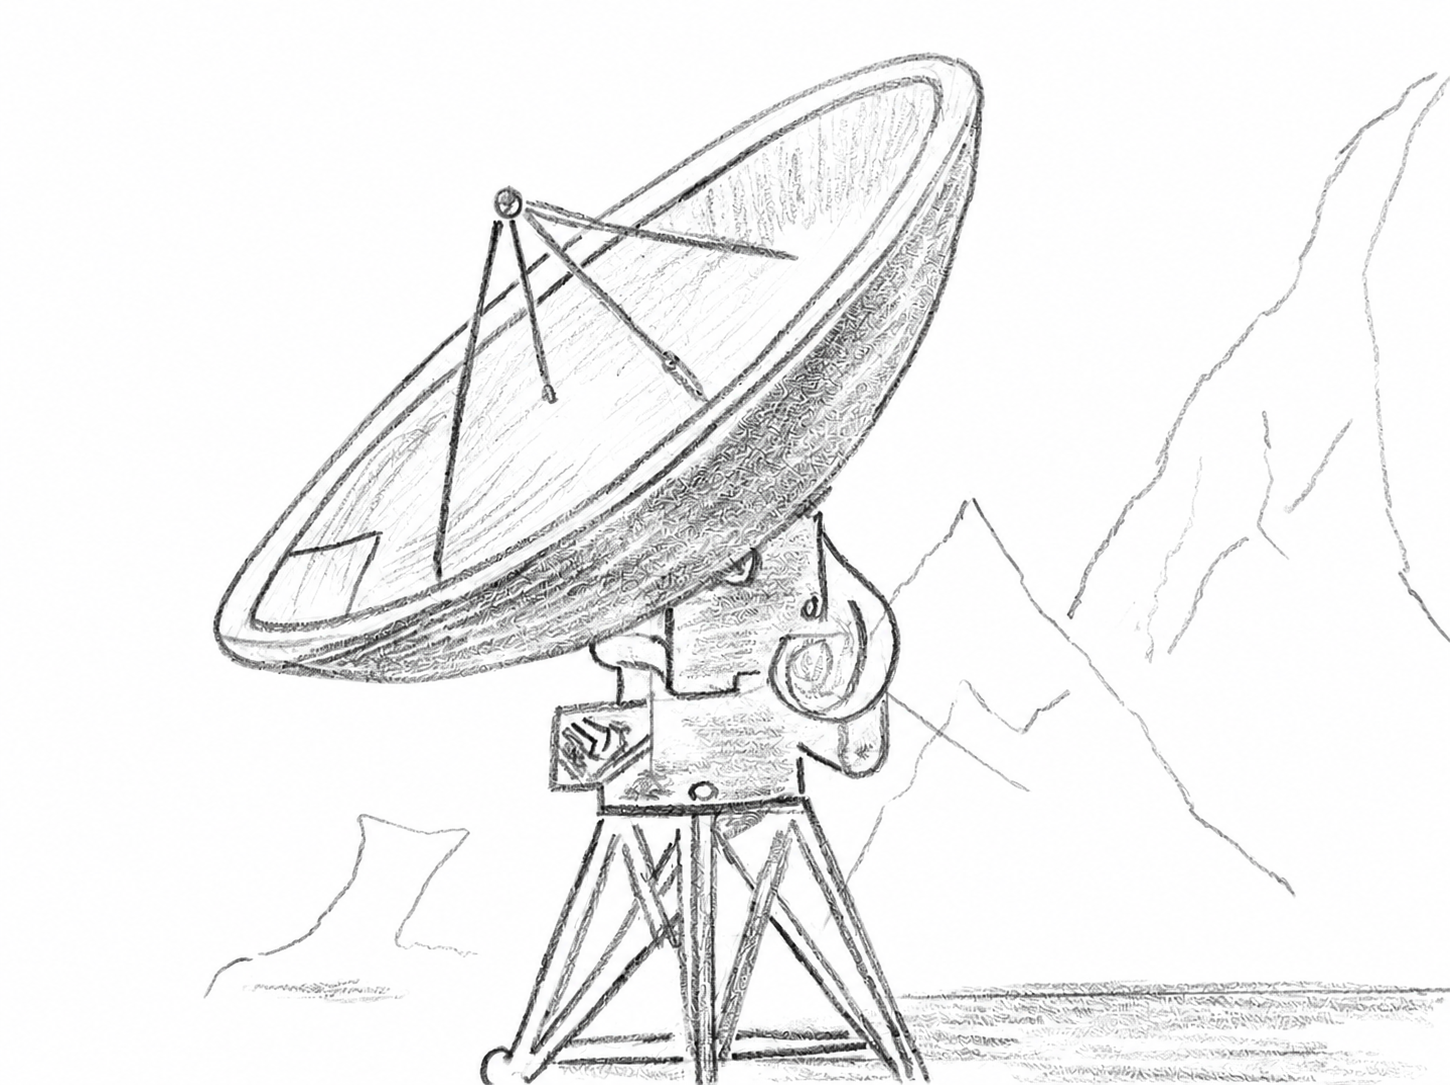
\includegraphics[width=0.39\paperwidth]{images/book-cover-bottom-right-hand-drawn-white.png}};

    \draw[
      step=10mm,
      draw=PolarisGrid,
      line width=0.16pt,
      opacity=0.55
    ] (current page.south west) grid (current page.north east);
  \end{tikzpicture}%
}

\renewcommand{\maketitle}{%
  \begin{titlepage}
    \thispagestyle{empty}
    \PolarisCoverSketches
    \centering

    \vspace*{0.31\textheight}

    \begin{minipage}{0.52\paperwidth}
      \centering
      {\PolarisTitleFont\fontsize{46}{54}\selectfont
       \MakeUppercase{\@title}\par}
    \end{minipage}

    \vspace{9mm}

    {\PolarisDivider\par}

    \vspace{5mm}

    \begin{minipage}{0.50\paperwidth}
      \centering
      {\fontsize{27}{31}\selectfont\@subtitle\par}
    \end{minipage}

    \vspace{16mm}

    {\fontsize{27}{31}\selectfont\@author\par}

    \vspace{5mm}

    {\fontsize{27}{31}\selectfont\@date\par}

    \vfill
  \end{titlepage}
}

% Show only the chapter title, not the automatic “Chapter 1” label.
\titleformat{\chapter}[display]
  {\normalfont\huge\bfseries}
  {}
  {0pt}
  {}

\makeatother
